% !TeX spellcheck = en_US
\newpage
\section{Physical}
In the network we have the \textbf{hosts}, end systems hosting user applications, and the \textbf{routers}, intermediate systems providing network connectivity.
\begin{center}
	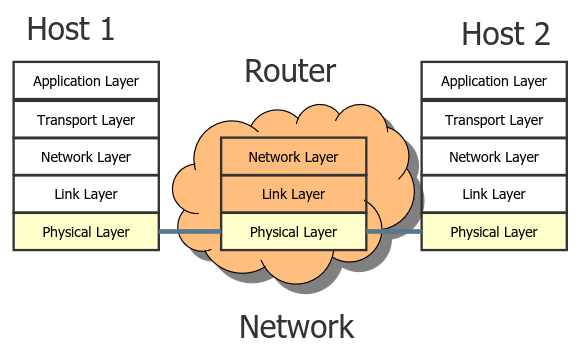
\includegraphics[scale=0.35]{ph}
\end{center}
The hosts have the full stack implementation while the routers only up to the Network Layer.
\subsection{Signals}
\begin{definition}[Signal]
	A signal is the physical representation of the data. It can be:
	\begin{itemize}
		\item \textbf{Analogue}: sequence of \textit{continuous} values
		\item \textbf{Digital}: sequence of \textit{discrete} values
	\end{itemize}
\end{definition}

Data is converted to signal which is then sent over the \textbf{transmission channel}, which is composed by \textbf{access points} and a \textbf{physical medium} (e.g. copper).
\begin{center}
	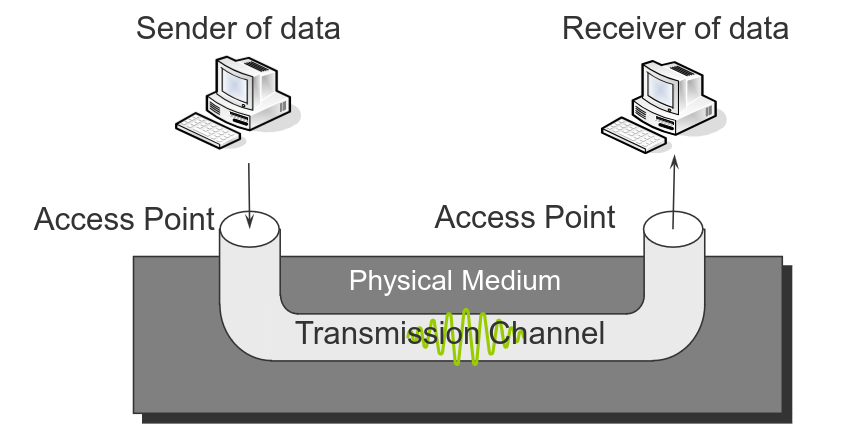
\includegraphics[scale=0.3]{phtr}
\end{center}
Since computers deal with digital signals, transmitting one bit via at a time a given medium, they need:
\begin{itemize}
	\item \textbf{Quantization}: convert from digital signal to analog signal and vice versa
	\item \textbf{Sampling}: must rely on periodical measurements of the physical medium
\end{itemize}
\begin{center}
	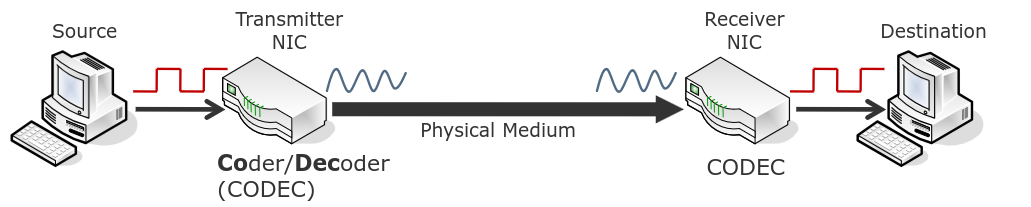
\includegraphics[scale=0.3]{codec}
\end{center}

\begin{observation}
	We have different challenges during the transmission of data:
	\begin{itemize}
		\item \textbf{Internal}: \textbf{collision} and \textbf{synchronization}
		\item \textbf{External}: \textbf{noise}
	\end{itemize}
\end{observation}

\newpage
\subsubsection{Periodic signal}
Periodic signals are the simplest signals. They take the following parameters:
\begin{itemize}
	\item \textbf{Period} $T$
	\item \textbf{Frequency} $f=\frac{1}{T}$
	\item \textbf{Amplitude} $S(t)$
	\item \textbf{Phase} $\varphi$
\end{itemize}

\begin{example}
	Some examples of signals:
	\begin{figure}[!h]
		\hfil
		\subfigure[Sine wave]{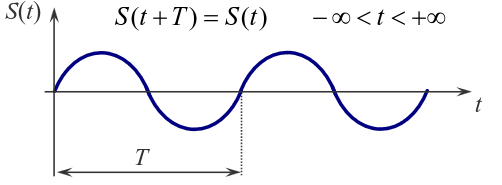
\includegraphics[scale=0.25]{sine}}
		\hfil
		\subfigure[Phase]{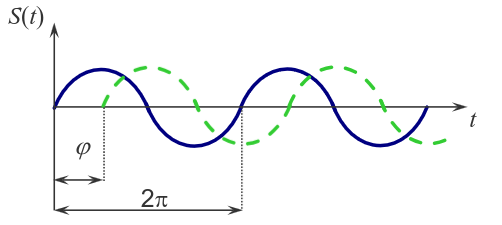
\includegraphics[scale=0.25]{phase}}
		\hfil
		\subfigure[Square wave]{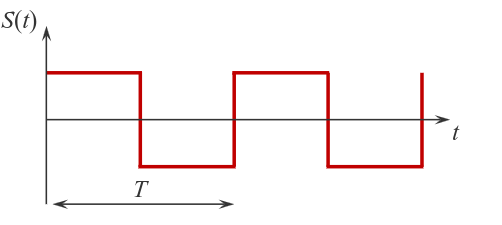
\includegraphics[scale=0.25]{square}}
	\end{figure}
\end{example}

\paragraph{Fourier Analysis} Like the composition of functions, it's possible to \textbf{compose} signals, generating new ones. In fact, per the \textbf{Fourier Analysis}, any period function can be constructed as the sum of a number of sines and cosines, resulting in a \textbf{Fourier Series}.
\begin{equation}
	g(t)=\frac{1}{2} c + \sum_{n=1}^{\infty} a_n \sin(2\pi nft) + \sum_{n=1}^{\infty}b_n \cos(2\pi nft)
\end{equation}
\textbf{Fourier Transform} is a mathematical transformation used to transform signals between time domain and frequency domain. Exists also in two dimensional space.
\paragraph{Distortion} If all Fourier components were equally diminished the resulting signal would be reduced in amplitude but not distorted. Unfortunately all transmission facilities diminish different components by different amounts, introducing \textbf{distortion}.

\paragraph{Frequency domain} The frequency domain is described by:
\begin{itemize}
	\item \textbf{Spectrum}: the range of frequencies a signals consists in
	\item \textbf{Bandwidth}: width of the \textit{spectrum}. In theory many signals have infinite bandwidth. The \textbf{effective bandwidth} is the narrow band of frequencies where most of the energy is contained.
\end{itemize}

\begin{example}
	In the following signal we have a \textbf{spectrum} from $f$ to $3f$ and a \textbf{bandwidth} of $2f$.
	\begin{figure}[!h]
		\hfil
		\subfigure[Time domain]{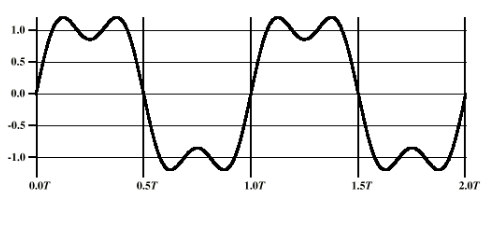
\includegraphics[scale=0.3]{time}}
		\hfil
		\subfigure[Frequency domain]{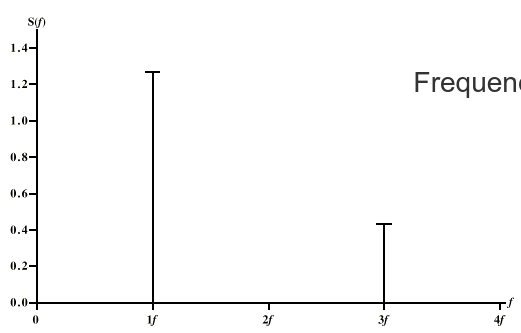
\includegraphics[scale=0.3]{freq}}
	\end{figure}
\end{example}

\subsubsection{Bandwidth}
We have two possible digital signal:
\begin{itemize}
	\item \textbf{Binary}: two possible values, $0$ and $1$
	\item \textbf{Multilevel}: more than two possible values (e.g. ternary, quaternary)
\end{itemize}
\begin{definition}[Symbol rate]
	Number of physical signaling events per unit of time on the transmission medium. The unit of measure is a \textbf{baud}.
\end{definition}
\begin{definition}[Data rate]
	Rate of bits decoded from symbol rate per unit of time. The unit of measure is $\frac{\text{bit}}{s}$. There are two cases:
	\begin{itemize}
		\item \textbf{Binary} signals with frequency $v$, each signaling event codes one bit
		\begin{equation*}
			\text{Data rate}=v
		\end{equation*}
		\item \textbf{Multilevel} signals with $n$ possible values
		\begin{equation*}
			\text{Data rate}=v \cdot \log_2(n)
		\end{equation*}
	\end{itemize}
\end{definition}

\begin{example}
	In this image we have a square wave with a negative ($0$) and a positive ($1$) pulse 
	\begin{center}
		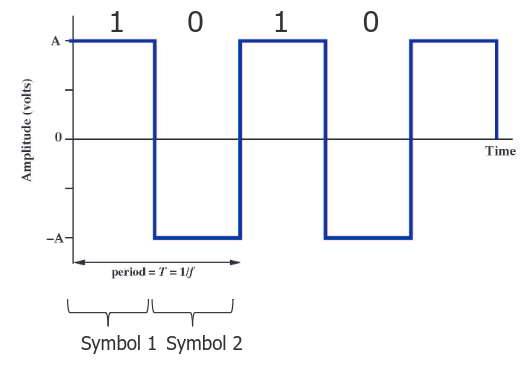
\includegraphics[scale=0.3]{bitrate}
	\end{center}
	The duration of a symbol is $\frac{1}{2} \cdot T = \frac{1}{2f}$, hence the \textbf{symbol rate} (which in this case is equal to the \textbf{data rate}) is $2f$ bits per second.
\end{example}

\begin{definition}[Bandwidth]
	The bandwidth of the medium is the highest $f_H$ minus lowest $f_L$ frequency which can be transmitted over this medium (in \textit{Hz}). $f_0$ is the center frequency.
	\begin{center}
		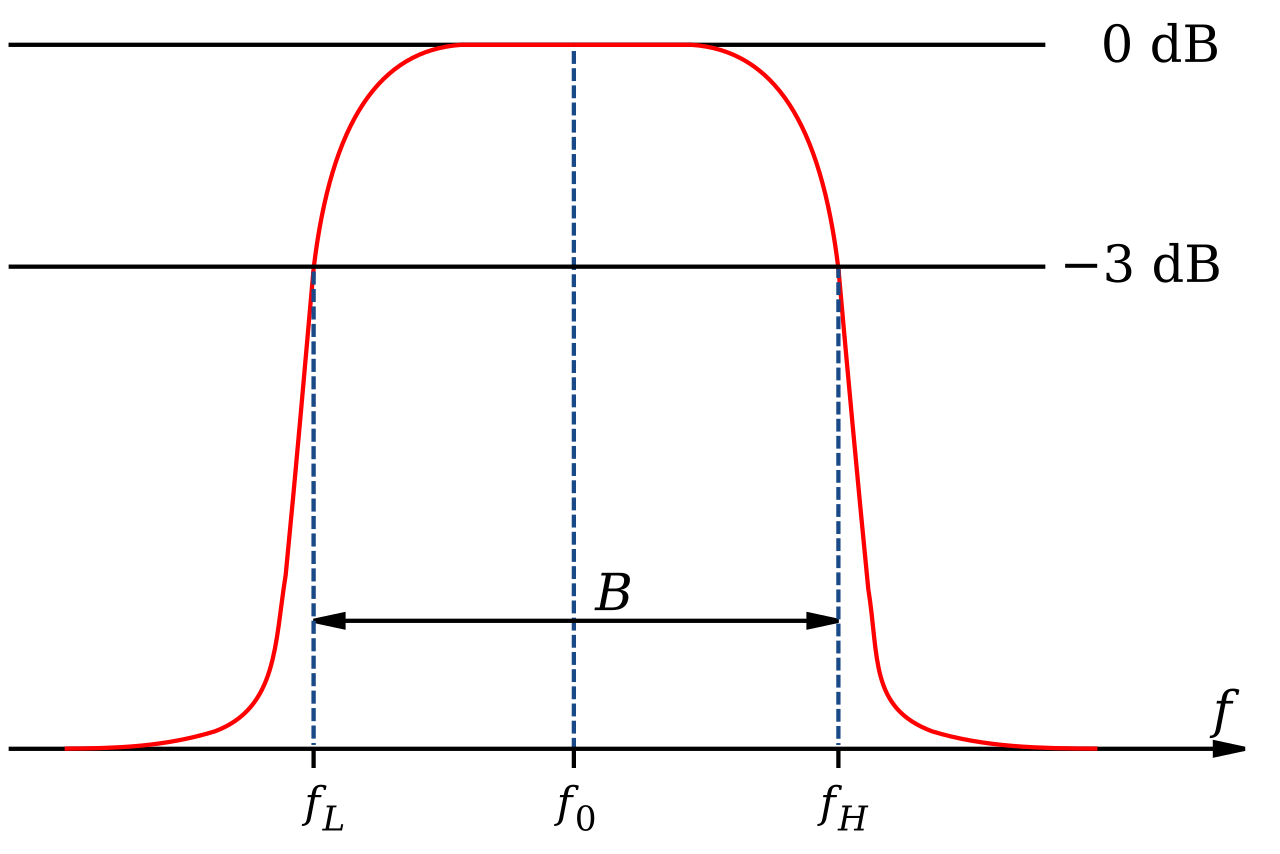
\includegraphics[scale=0.1]{bw}
	\end{center}
\end{definition}
A \textbf{square wave} is composed of an infinite number of \textbf{harmonics}, where the amplitude of the $k$th one is $\frac{1}{k}$.
\begin{equation}
	s(t)=A \cdot \frac{4}{\pi}\cdot\sum_{k=1, k \text{ odd}}^{\infty}\frac{1}{k}\sin(2\pi kft)
\end{equation}
While theoretically we would need an infinite bandwidth to get a square wave, the medium limits the number of harmonics.
\subsection{Transmission}
The fundamental problem of communication consists in reproducing on one side exactly or approximated a message selected on the other side. The ideal transmission would be a square wave while the actual one is an approximation.\\
To get from an analog to a digital signal, there are two main operations:
\begin{itemize}
	\item \textbf{Quantization}: from a continuous value we get a discrete one with an error
	\item \textbf{Sampling}: periodical measures at a given rate with an interval $T$
	\begin{theorem}[Nyquist Sampling Theorem]
		To allow the reconstruction of the original analog signal it is sufficient that the sampling frequency $f_s$ is such that
		\begin{equation}
			f_s > 2W
		\end{equation}
		where $W$ is the bandwidth in Hz.
	\end{theorem}
\end{itemize}

\begin{center}
	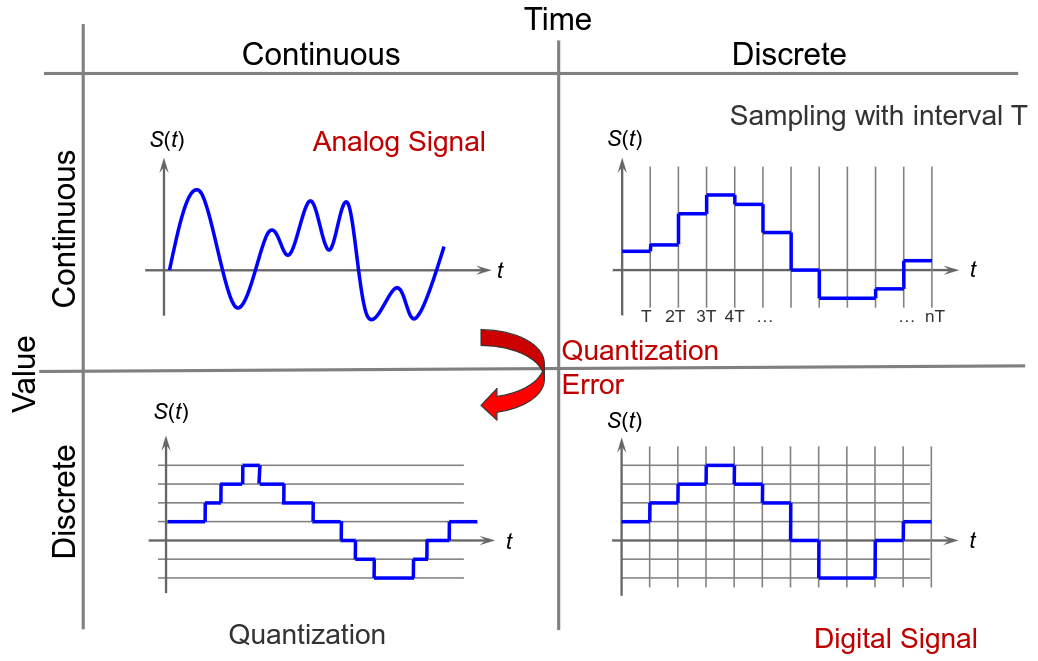
\includegraphics[scale=0.3]{andig}
\end{center}
To get an analog signal from a digital one we perform the \textbf{coding} operation, where the quantization intervals are assigned to a binary code and then transmitted.

\subsubsection{Channel capacity}
To define the \textbf{capacity} of an analog physical channel, we need to consider that there is always some \textbf{noise}. This means that the capacity will be \textbf{finite} and will depend on several parameters, usually:
\begin{itemize}
	\item \textbf{Additive}: the noise value is added to the signal and that's what the receiver gets
	\item \textbf{White noise}: independent, random noise values with constant spectral density
	\item \textbf{Gaussian}: probability distribution of the amplitude of random noise values
\end{itemize}
While on the analog signals noise will cause degradation of the quality, on digital ones it causes \textbf{bit errors}. It is possible to reduce the effect of noise by boosting signal amplitude, but requires energy and causes more interferences.\\ \textbf{Transmission impairments} essentially come from:
\begin{itemize}
	\item Signal \textbf{attenuation} and \textbf{attenuation distortion}
	\item \textbf{Delay distortion}
	\item \textbf{Noise}
	\begin{itemize}
		\item \textit{Thermal} noise
		\item \textit{Intermodulation} noise
		\item \textit{Crosstalk}
		\item \textit{Impulse} noise
	\end{itemize}
\end{itemize}
\newpage
\begin{definition}[BER]
	Bit Error Rate is a metric for bit errors. It depends on the \textbf{environment}, on the \textbf{communication medium} and the \textbf{length} of the transmission line (higher frequencies attenuated stronger than lower, different frequencies have different speed).
	\begin{equation}
		\text{BER} = \frac{\text{Number of erroneous bits}}{\text{Number of transmitted bits}}
	\end{equation}
\end{definition}
\begin{theorem}[Shannon Theorem]
	A channel with $W$ bandwidth, $P$ average signal power and $N$ average noise power has a maximum data rate of:
	\begin{equation}
		\text{maximum data rate} = W \cdot \log_2(1+\underbrace{\frac{P}{N}}_{\text{SNR\footnotemark}})
	\end{equation}
\end{theorem}

\footnotetext{Signal to Noise Ratio}

\noindent Even if we don't consider noise, throughput is still \textbf{finite} due to:
\begin{itemize}
	\item \textbf{Quantization} at the transmitter and \textbf{discrete levels} of the signals
	\item \textbf{Sampling} at the receiver
\end{itemize}
While Shannon Theorem gives us an upper bound for the data rate, we can use Nyquist theorem to calculate the amount of discrete signals needed to achieve that.
\begin{theorem}[Nyquist theorem]
	Given a channel of $W$ bandwidth and $n$ discrete levels of the signal, the maximum data rate is
	\begin{equation}
		\text{maximum data rate} = 2W \cdot \log_2(n)
	\end{equation}
\end{theorem}

\subsection{Data encoding}
To transmit individual bits there are two options:
\begin{itemize}
	\item \textbf{Baseband}: the original data is transmitted "as is" over the medium, requiring \textbf{data encoding}
	\item \textbf{Broadband}: the data is transmitted by \textbf{modulating} it onto a \textbf{carrier} analog signal
\end{itemize}
A data encoding technique needs:
\begin{itemize}
	\item \textbf{Robustness}: tolerance to distortion
	\item \textbf{Efficiency}: high transmission rate, achieved using coded words (binary, ternary, quaternary)
	\item \textbf{Synchronization} with receiver: less opportunities for out-of-sync. Achieved by frequent changes of voltage level regarding to a fixed cycle. Needs to avoid direct current: positive and negative signals should alternatively arise. Bipolar/Unipolar encoding.
\end{itemize}

\subsubsection{NRZ}
Non Return to Zero is a simple approach where $1$ is coded with a positive voltage ($+5V$) and $0$ 	as a negative one ($-5V$). It's very \textbf{simple} and the smaller the clock pulse, the higher the data rate. It's prone to \textbf{loss of synchronization} and has \textbf{direct current} during long sequences of the same bit.
\begin{center}
	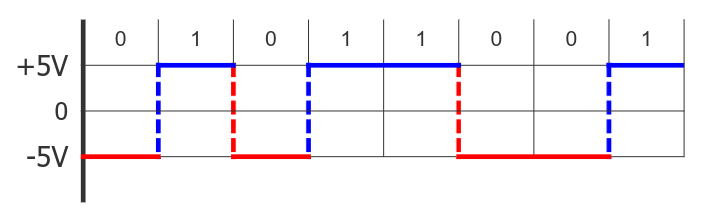
\includegraphics[scale=0.3]{nrz}
\end{center}

\subsubsection{RZ}
Return to zero works on the same principle of NRZ but after each bit the signal goes back to zero first. This way, the signal is \textbf{self-clocking} and there is no direct current. It needs twice the bandwidth.
\begin{center}
	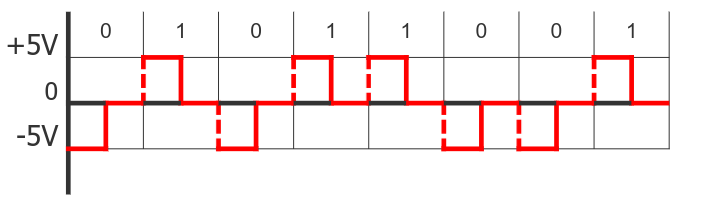
\includegraphics[scale=0.3]{rz}
\end{center}

\subsubsection{Differential NRZ}
Similar principle of NRZ but $1$ is encoded as a \textbf{voltage level change} and $0$ as a missing change, thus having the disadvantages of NRZ only for a sequence of zeros.
\begin{center}
	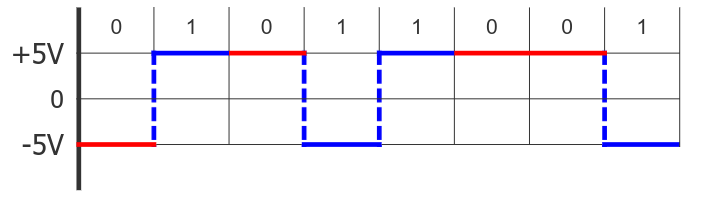
\includegraphics[scale=0.3]{dnrz}
\end{center}

\subsubsection{Manchester code}
With each code element the clock pulse is transferred: voltage level change occurs in the middle of each bit. $0$ is encoded as voltage level change from positive ($+5V$) to negative ($-5V$) while $1$ as voltage level change from negative ($-5V$) to positive ($+5V$).\\
Clock synchronization happens for each bit and the end of the transmission is easily recognizable. The capacity used is only half.
\begin{center}
	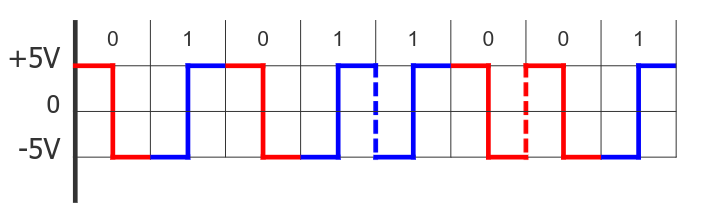
\includegraphics[scale=0.3]{mch}
\end{center}

\subsubsection{Differential Manchester code}
A variant of the Manchester code. $0$ is encoded as a voltage level change while $1$ as a missing one.
\begin{center}
	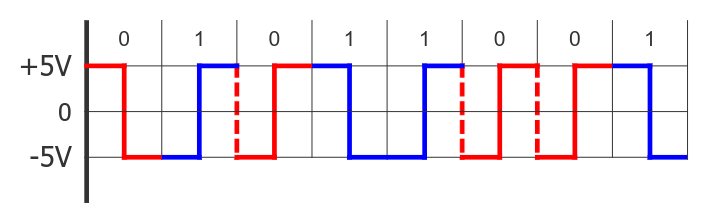
\includegraphics[scale=0.3]{dmch}
\end{center}

\subsubsection{4B/5B}
\begin{wrapfigure}[7]{r}{3.2cm}
	\vspace{-1.5cm}
	\begin{center}
		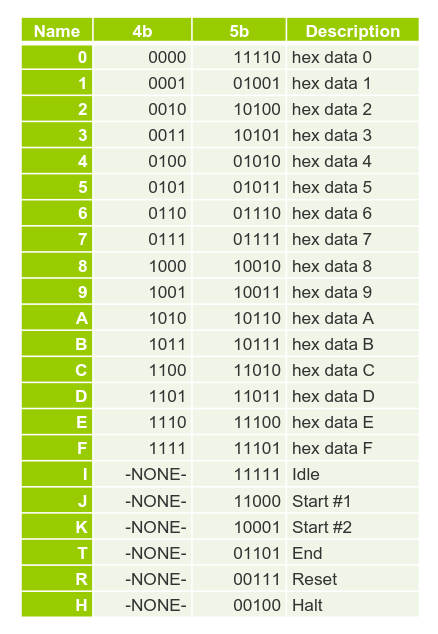
\includegraphics[width=3.2cm]{4b5b}
	\end{center}
\end{wrapfigure}
To improve the efficiency of the Manchester code, this techniques codes a hexadecimal character of four bits in five, avoiding long zero blocks. Uses the same principle of the differential NRZ. Allows some combinations for control information. The transmission provides clocking.\\
It's used in the USB and FastEthernet context and in GigabitEthernet with different variants (8B/10B, 64B/66B, $\ldots$).

\subsection{Modulation}
To transmit with \textbf{broadband} we need to modulate the signal, that being \textbf{shaping} a carrier frequency via the baseband signal.
\begin{equation}
	s(t) = A \cdot \sin(2 \cdot \pi f t + \varphi)
\end{equation}
\subsubsection{ASK}
Modulation of the \textbf{amplitude} $A$. It's easy to realize and doesn't need much bandwidth but it's not robust against distortions. Often used in optical transmissions.
\begin{center}
	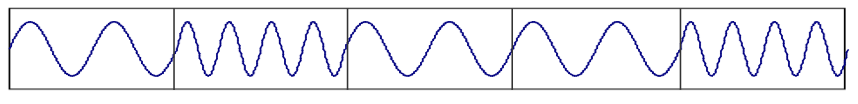
\includegraphics[scale=0.15]{ask}
\end{center}

\subsubsection{FSK}
Modulation of the \textbf{frequency} $f$. It was the first used in data transmission using phone lines. Needs a lot of bandwidth and it's a waste of frequencies.
\begin{center}
	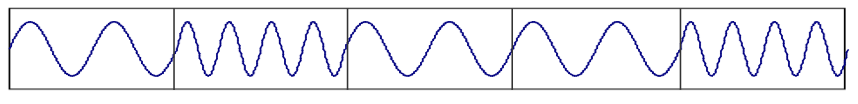
\includegraphics[scale=0.15]{fsk}
\end{center}

\subsubsection{PSK}
Modulation of the \textbf{phase} $\varphi$. It has a complex demodulation process but it's robust against disturbances.
\begin{center}
	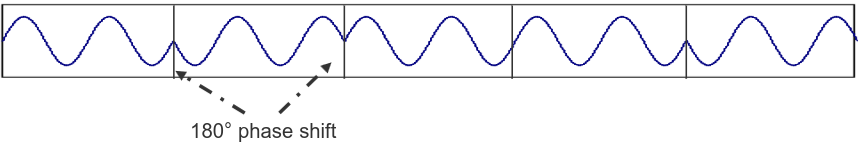
\includegraphics[scale=0.15]{psk}
\end{center}
Also called \textbf{Binary} PSK.

\subsubsection{PSK variants}
\textbf{Quadrature Phase Shifting Key} (also 2B1Q) allows the shifting between $4$ phases, allowing for $4$ states and thus $2$ bits at a time (doubling the data rate).
\begin{center}
	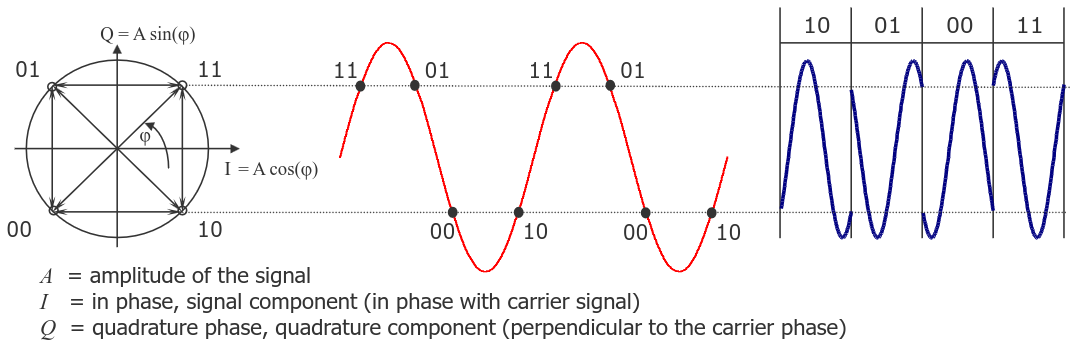
\includegraphics[scale=0.25]{qpsk}
\end{center}
\textbf{Differential} BPSK works with two different phases like PSK but it shifts only if $1$ is the next bit.
\begin{center}
	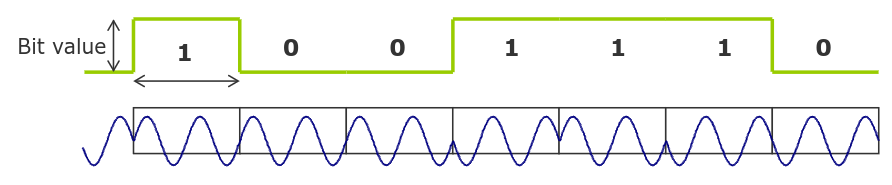
\includegraphics[scale=0.25]{dbpsk}
\end{center}
\textbf{Quadrature Amplitude Modulation} is a combination of ASK and QPSK. $n >2$ bit can be transferred at the same time. Bit error rate increases with $n$ but is still less than similar techniques. Used frequently in wireless communication.
\begin{center}
	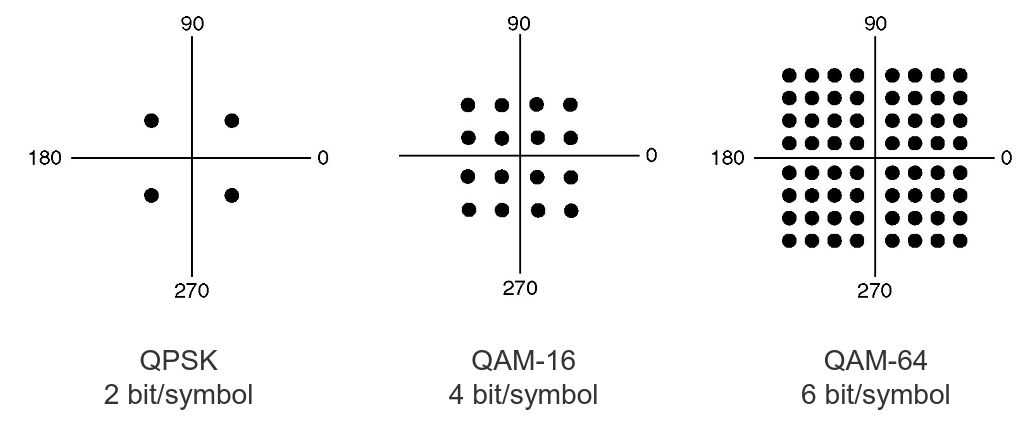
\includegraphics[scale=0.2]{qam}
\end{center}

\subsection{Multiplexing}
Since lines are expensive it's important to share the resources. Multiplexing is a technique that provides simultaneous transmission over a single medium.\\
\begin{wrapfigure}[7]{r}{5cm}
	\begin{center}
		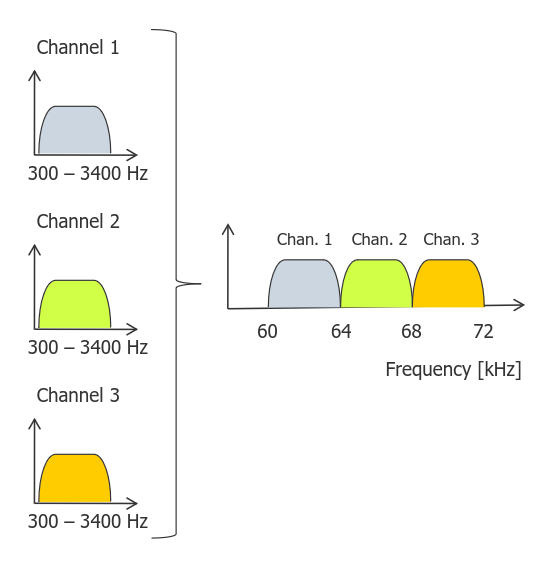
\includegraphics[width=5cm]{fdm}
	\end{center}
\end{wrapfigure}
\subsubsection{FDM}
\textbf{Frequency} Division Multiplexing divides the frequency spectrum in frequency \textbf{bands}, which are used exclusively and simultaneously. When used for optical transmission is called \textbf{Wavelength Division Multiplexing}.
\begin{center}
	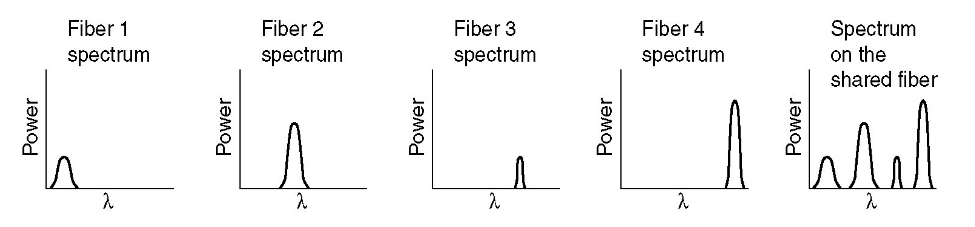
\includegraphics[scale=0.2]{wdm}
\end{center}

\subsubsection{TDM}
\textbf{Time} Division Multiplexing divides time into slots of fixed or variable length. Each timeslot represents one sub-channel.
\begin{center}
	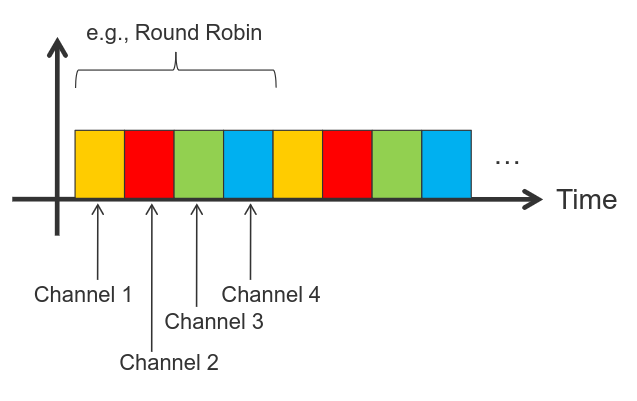
\includegraphics[scale=0.3]{tdm}
\end{center}
A classical TDM is the T1, having $24$ channels in parallel with $8$bit per channel (one is control), a $193$ bit frame that lasts for $125\mu$sec for $1.554$Mbit/s.
\begin{center}
	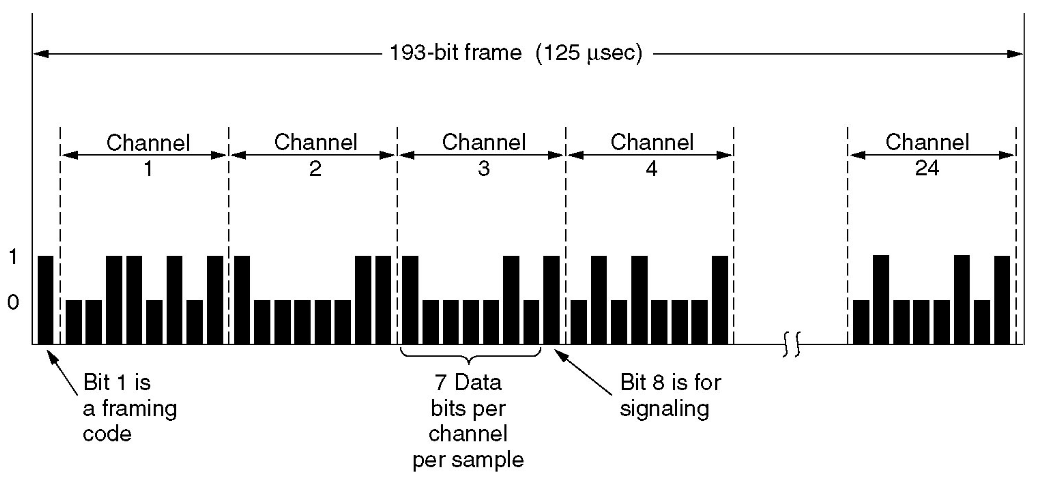
\includegraphics[scale=0.3]{t1}
\end{center}
It's possible to multiplex T1 into higher carriers to get T2, T3, $\ldots$.

\begin{note}
	Multiplexing techniques plus algorithm that control how to do it result in \textbf{Multiple Access} technologies (e.g. FDMA, TDMA) on layer 2.
\end{note}

\newpage
\subsection{Physical media}
There are many different \textbf{medias}.
\begin{center}
	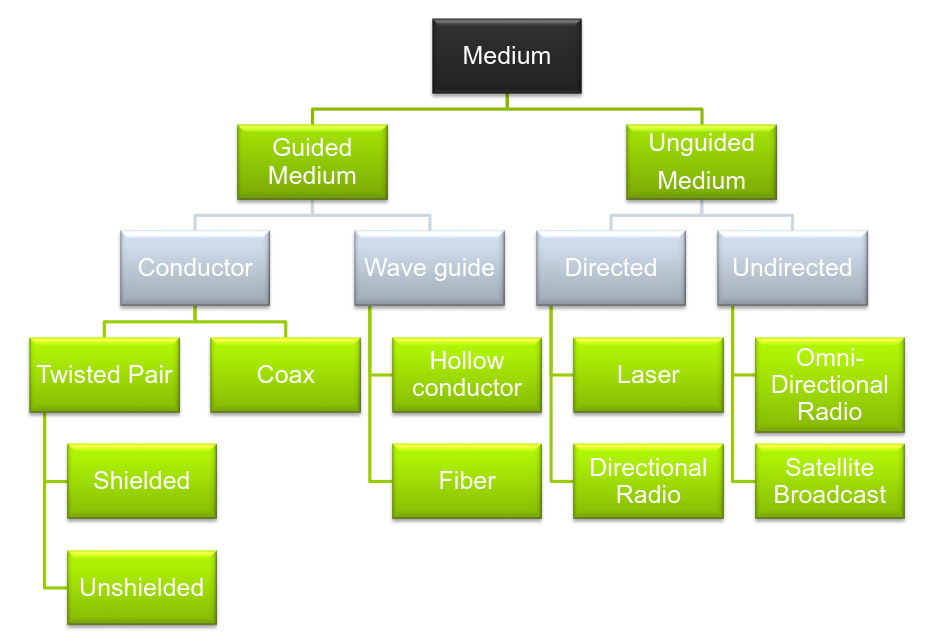
\includegraphics[scale=0.3]{class}
\end{center}
And different type of \textbf{networks}, classified over the size of their scope.
\begin{table}[!h]
	\centering
	\begin{tabular}{|c|c|c|}
		\hline
		\textbf{Name} & \textbf{Scope} & \textbf{Example} \\
		\hline
		\textit{Body/Personal} & 1mt & Body \\
		\hline
		\textit{Local} & 10mt-100mt & Room, Building \\
		\hline
		\textit{Metropolitan} & 1Km-10Km & Campus, Town \\
		\hline
		\textit{Wide} & 100Km-1000Km & Country, Continent \\
		\hline
		\textit{Internet} & 10000Km & Planet \\
		\hline
	\end{tabular}
\end{table}
\subsubsection{Electromagnetic waves}
Electromagnetic waves are used to transmit the signal over cables and wireless. In a vacuum they travel at the speed of light $c$ but in copper or fiber they slow down at about $\frac{2}{3}$ of $c$.\\
The \textbf{fundamental relationship} between wavelength $\lambda$, frequency $f$ and $c$:
\begin{equation}
	\lambda \cdot f = c
\end{equation}

\subsubsection{Guided medium}
\begin{wrapfigure}[7]{r}{3.2cm}
	\vspace{-1cm}
	\begin{center}
		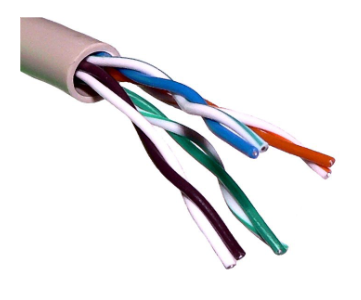
\includegraphics[width=3.2cm]{cable}
	\end{center}
\end{wrapfigure}
\paragraph{Twisted pair} This medium transmits data through \textbf{electrical signals}. Electromagnetic signals from the environment can disturb it, thus it's necessary to have \textbf{insulation} and \textbf{twisting} (also done at different rates to reduce \textbf{crosstalk}). It's cheap and simple and it's used both for digital and analog signals. They have a bit-error rate of $\approx 10^{-5}$.\\
They are divided in:
\begin{itemize}
	\item \textbf{Unshielded} (U)
	\item \textbf{Foil shielded} (F)
	\item \textbf{Screen shielded} (S)
\end{itemize}
The \textbf{shield} can be individual, overall or both. They are also divided in \textbf{categories} based on their shielding level and maximum speed.
\paragraph{Coaxial}
It's a copper cable with braided outer conductor to reduce disturbances and interior insulation between them. Has a bit-rate error of $\approx 10^{-9}$, has higher data rates over longer distances compared to the twisted pair and has a better signal quality.
\begin{center}
	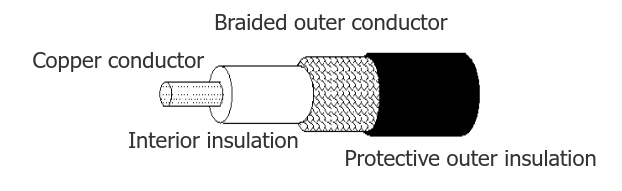
\includegraphics[scale=0.3]{coax}
\end{center}

\paragraph{Optical Fiber}
\begin{wrapfigure}[5]{r}{3.2cm}
	\vspace{-0.5cm}
	\begin{center}
		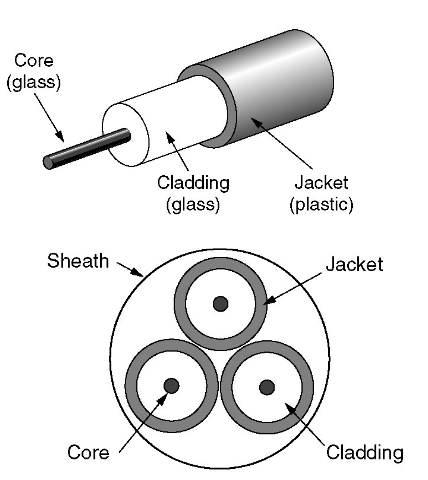
\includegraphics[width=3.2cm]{fibercable}
	\end{center}
\end{wrapfigure}
Huge capacity with nearly unlimited data rate. It's insensitive to electromagnetic disturbances. Has a good signal-to-noise ratio. It's smaller and lighter and has a bit-error rate of $\approx 10^{-12}$.\\
The structure of an optical transmission system has:
\begin{itemize}
	\item \textbf{Light source}: converts electrical into optical signals, $1$ is a light pulse and $0$ is no light pulse
	\item \textbf{Transmission medium}, the optical fiber
	\item \textbf{Detector}: converts optical into electrical signals
\end{itemize}
\begin{center}
	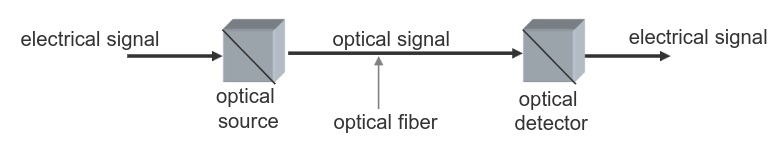
\includegraphics[scale=0.3]{fiber}
\end{center}
The cable has a \textbf{core} made of optical glass (super thin), an internal \textbf{glass cladding} and a protective \textbf{plastic covering}. The transmission takes place in the core, which has a high \textbf{refractive index} (refraction effect relatively to vacuum), where a ray of light is reflected between the two mediums.
\begin{center}
	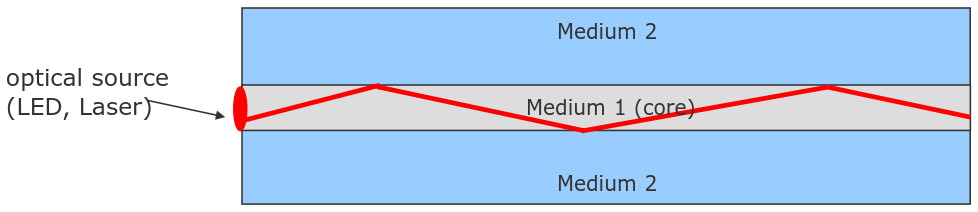
\includegraphics[scale=0.25]{fiberphoto}
\end{center}
There are three types of fiber cables:
\begin{itemize}
	\item \textbf{Single mode}: with a diameter core of $8-10\mu m$, all rays can go in only one direction and therefore having no dispersion (homogeneous signal delay). Expensive due to small core.
	\begin{center}
		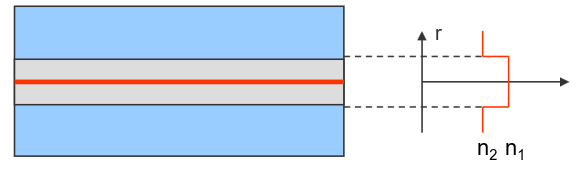
\includegraphics[scale=0.3]{single}
	\end{center}
	\item \textbf{Simple multimode} (step index): core diameter of $50\mu m$, uses different wavelengths with different delay signals and therefore has a high dispersion
	\begin{center}
		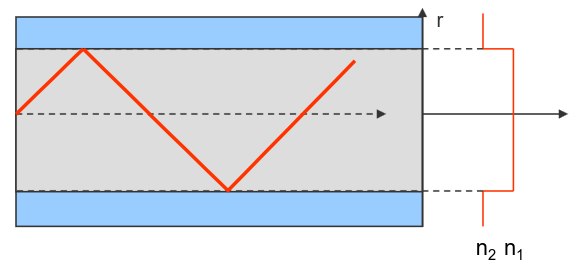
\includegraphics[scale=0.3]{smulti}
	\end{center}
	\newpage
	\item \textbf{Multimode} with gradient index: same as the simple multimode but the refracting index changes continuously, hence having a low dispersion
	\begin{center}
		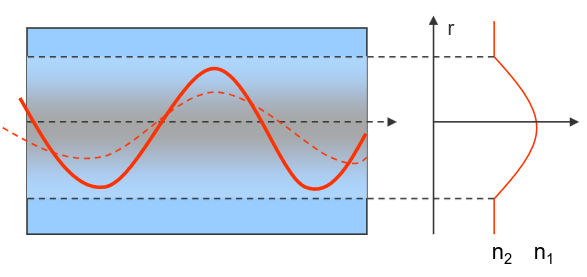
\includegraphics[scale=0.3]{multi}
	\end{center}
\end{itemize}

\paragraph{Radiation sources} Radiation sources can be of two types:
\begin{itemize}
	\item \textbf{LED}: cheap and reliable, has a broad wavelength spectrum thus a \textbf{high dispersion} (small range) and a \textbf{low capacity}
	\item \textbf{Laser}: \textbf{expensive} but with \textbf{high capacity} and a small wavelength spectrum and thus \textbf{high range}. They  are sensitive to \textbf{temperatures}.
\end{itemize}
On the other side of the signals there are \textbf{photodiodes}.

\paragraph{Attenuation} The ray of light is increasingly weakened along the medium due to \textbf{absorption} and \textbf{impurities} in it.

\paragraph{Dispersion} Rays of light spread in the medium at different speeds, refractive index in the medium is not constant.

\subsubsection{Home connection}
There are multiple solutions to connect homes to the internet:
\begin{itemize}
	\item Existing \textbf{phone lines} local loop (DSL). It was the first approach. It needed a MoDem (Modulator and Demodulator) to convert digital data into analogs and viceversa. Today uses the whole spectrum of the copper cable and modulates through \textbf{Discrete Multi-Tone} or \textbf{Carrierless Amplitude Phase}. Calls are now over IP. The main standards are VDSL and VDSL2
	\item Existing \textbf{cable TV} network connections, using coaxial and upstream multiplexing through \textbf{Cable Modem Termination System}. Uses the \textbf{DOCSIS} standard.
	\item Deployed \textbf{cellular networks}
	\item Existing \textbf{powerline connections}
	\item \textbf{Satellite} communication
	\item \textbf{Microwave} links
	\item \textbf{Fiber-to-the-home}
\end{itemize}

\paragraph{Discrete Multi-Tone Modulation}
Uses multiple carriers where each channel uses a suitable optimal modulation method (QAM). Channels in high frequencies have a lower quality over long distances.
\begin{center}
	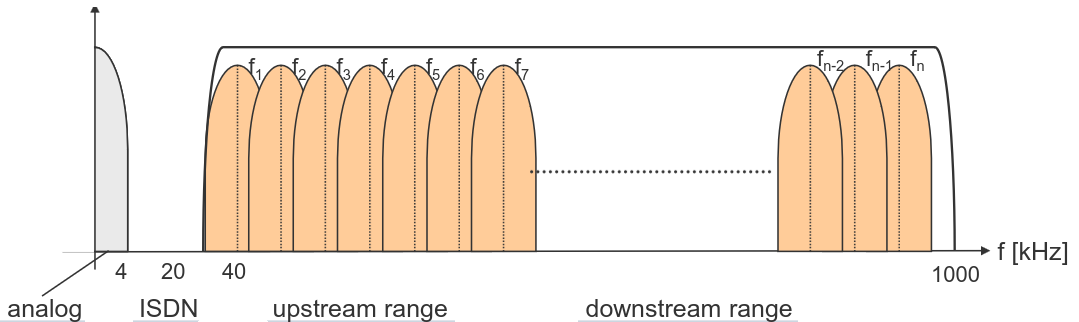
\includegraphics[scale=0.3]{dmt}
\end{center}